%!TEX root = ../master.tex
\chapter{Discussion}\label{ch:discussion}
This chapter contains discussion of the entire project 

\section{Sources of error}

\todo{ ved ikke hvor jeg skal skrive det her, men det kommer lige her, skal sættes ind det rette sted og rettes i}
 Since the final test were only conducted on 14 medialogy students and one Art \& technology student, is it hard to say if our product would be just as "easy to understand" for a normal museum visitor or any other user. To investigate if the product would be accepted among people with no knowledge of audio processing or people who are having trouble understanding "technical stuff I don't know" the optimal solution would be to test the product in context, in this case it could be at an art museum, where the test would be conducted on guests of the museum which could be people of all age groups. 
 
 \section{Contex of use}
During this project, two of the members of the project group spend a day visiting the art museum Kunsten in Aalborg. The goal was to find out how the artefact could be used in context at the museum. With the non finished product in mind, the group members studied the different art exhibitions and tried to imagine the product in context with the art. 

During the visit, more exhibition were found and studied, however the main inspiration for context of use were limited to three pictures \ref{Fig:Kblod} , \ref{Fig:aftryk} and \ref{Fig:aftryk} These images were used to create sketches of the project artefact as a set up in an art museum as seen in \ref{Fig:productsetupsketch}

\begin{figure}[!h] 
\centering
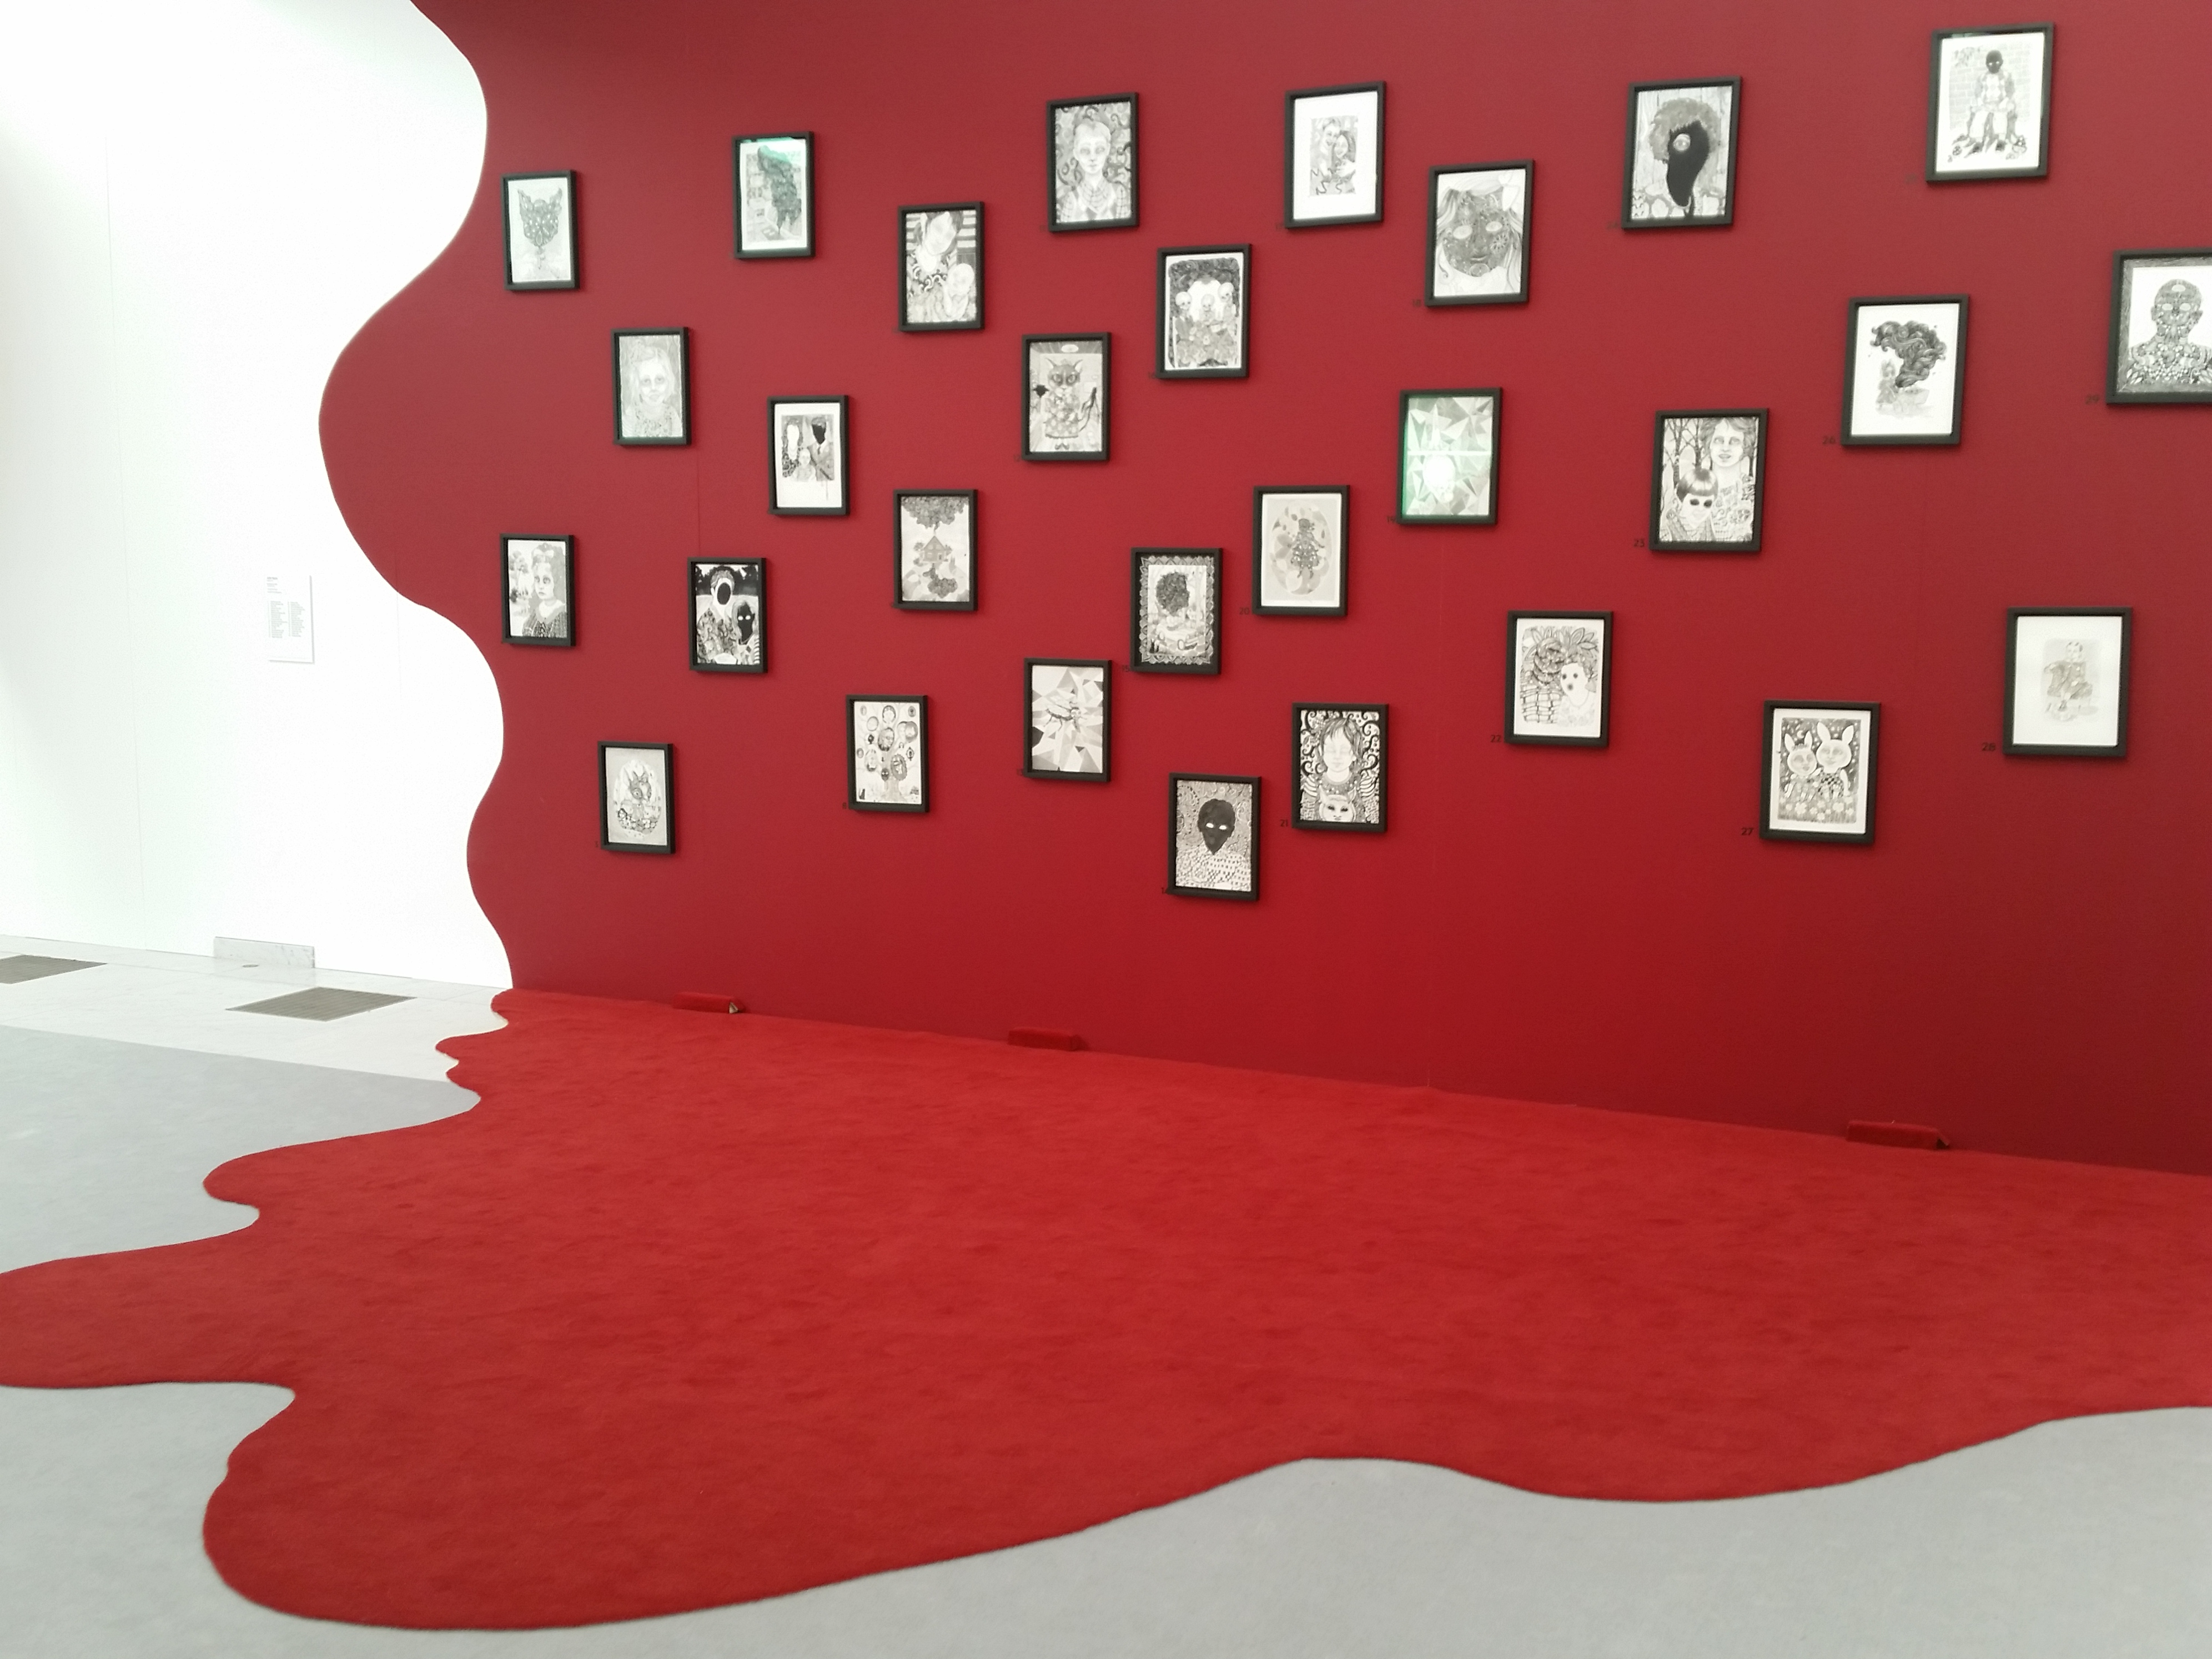
\includegraphics[width=1\textwidth]{Kblod}
\caption{\label{fig:Kblod} Picture taken from Kunsten.}
\end{figure}
The art piece creates a connection between the wall and floor with the red carpet. Inspiration were taken from this piece because the red colour of the floor and wall indicates that the two are connected, the project group saw a need to make it clear that the painting and the artefact were connected, therefore a sketch were a colour connects the artefact to the painting as seen in \ref{Fig:productsetupsketch}


\begin{figure}[!h] 
\centering
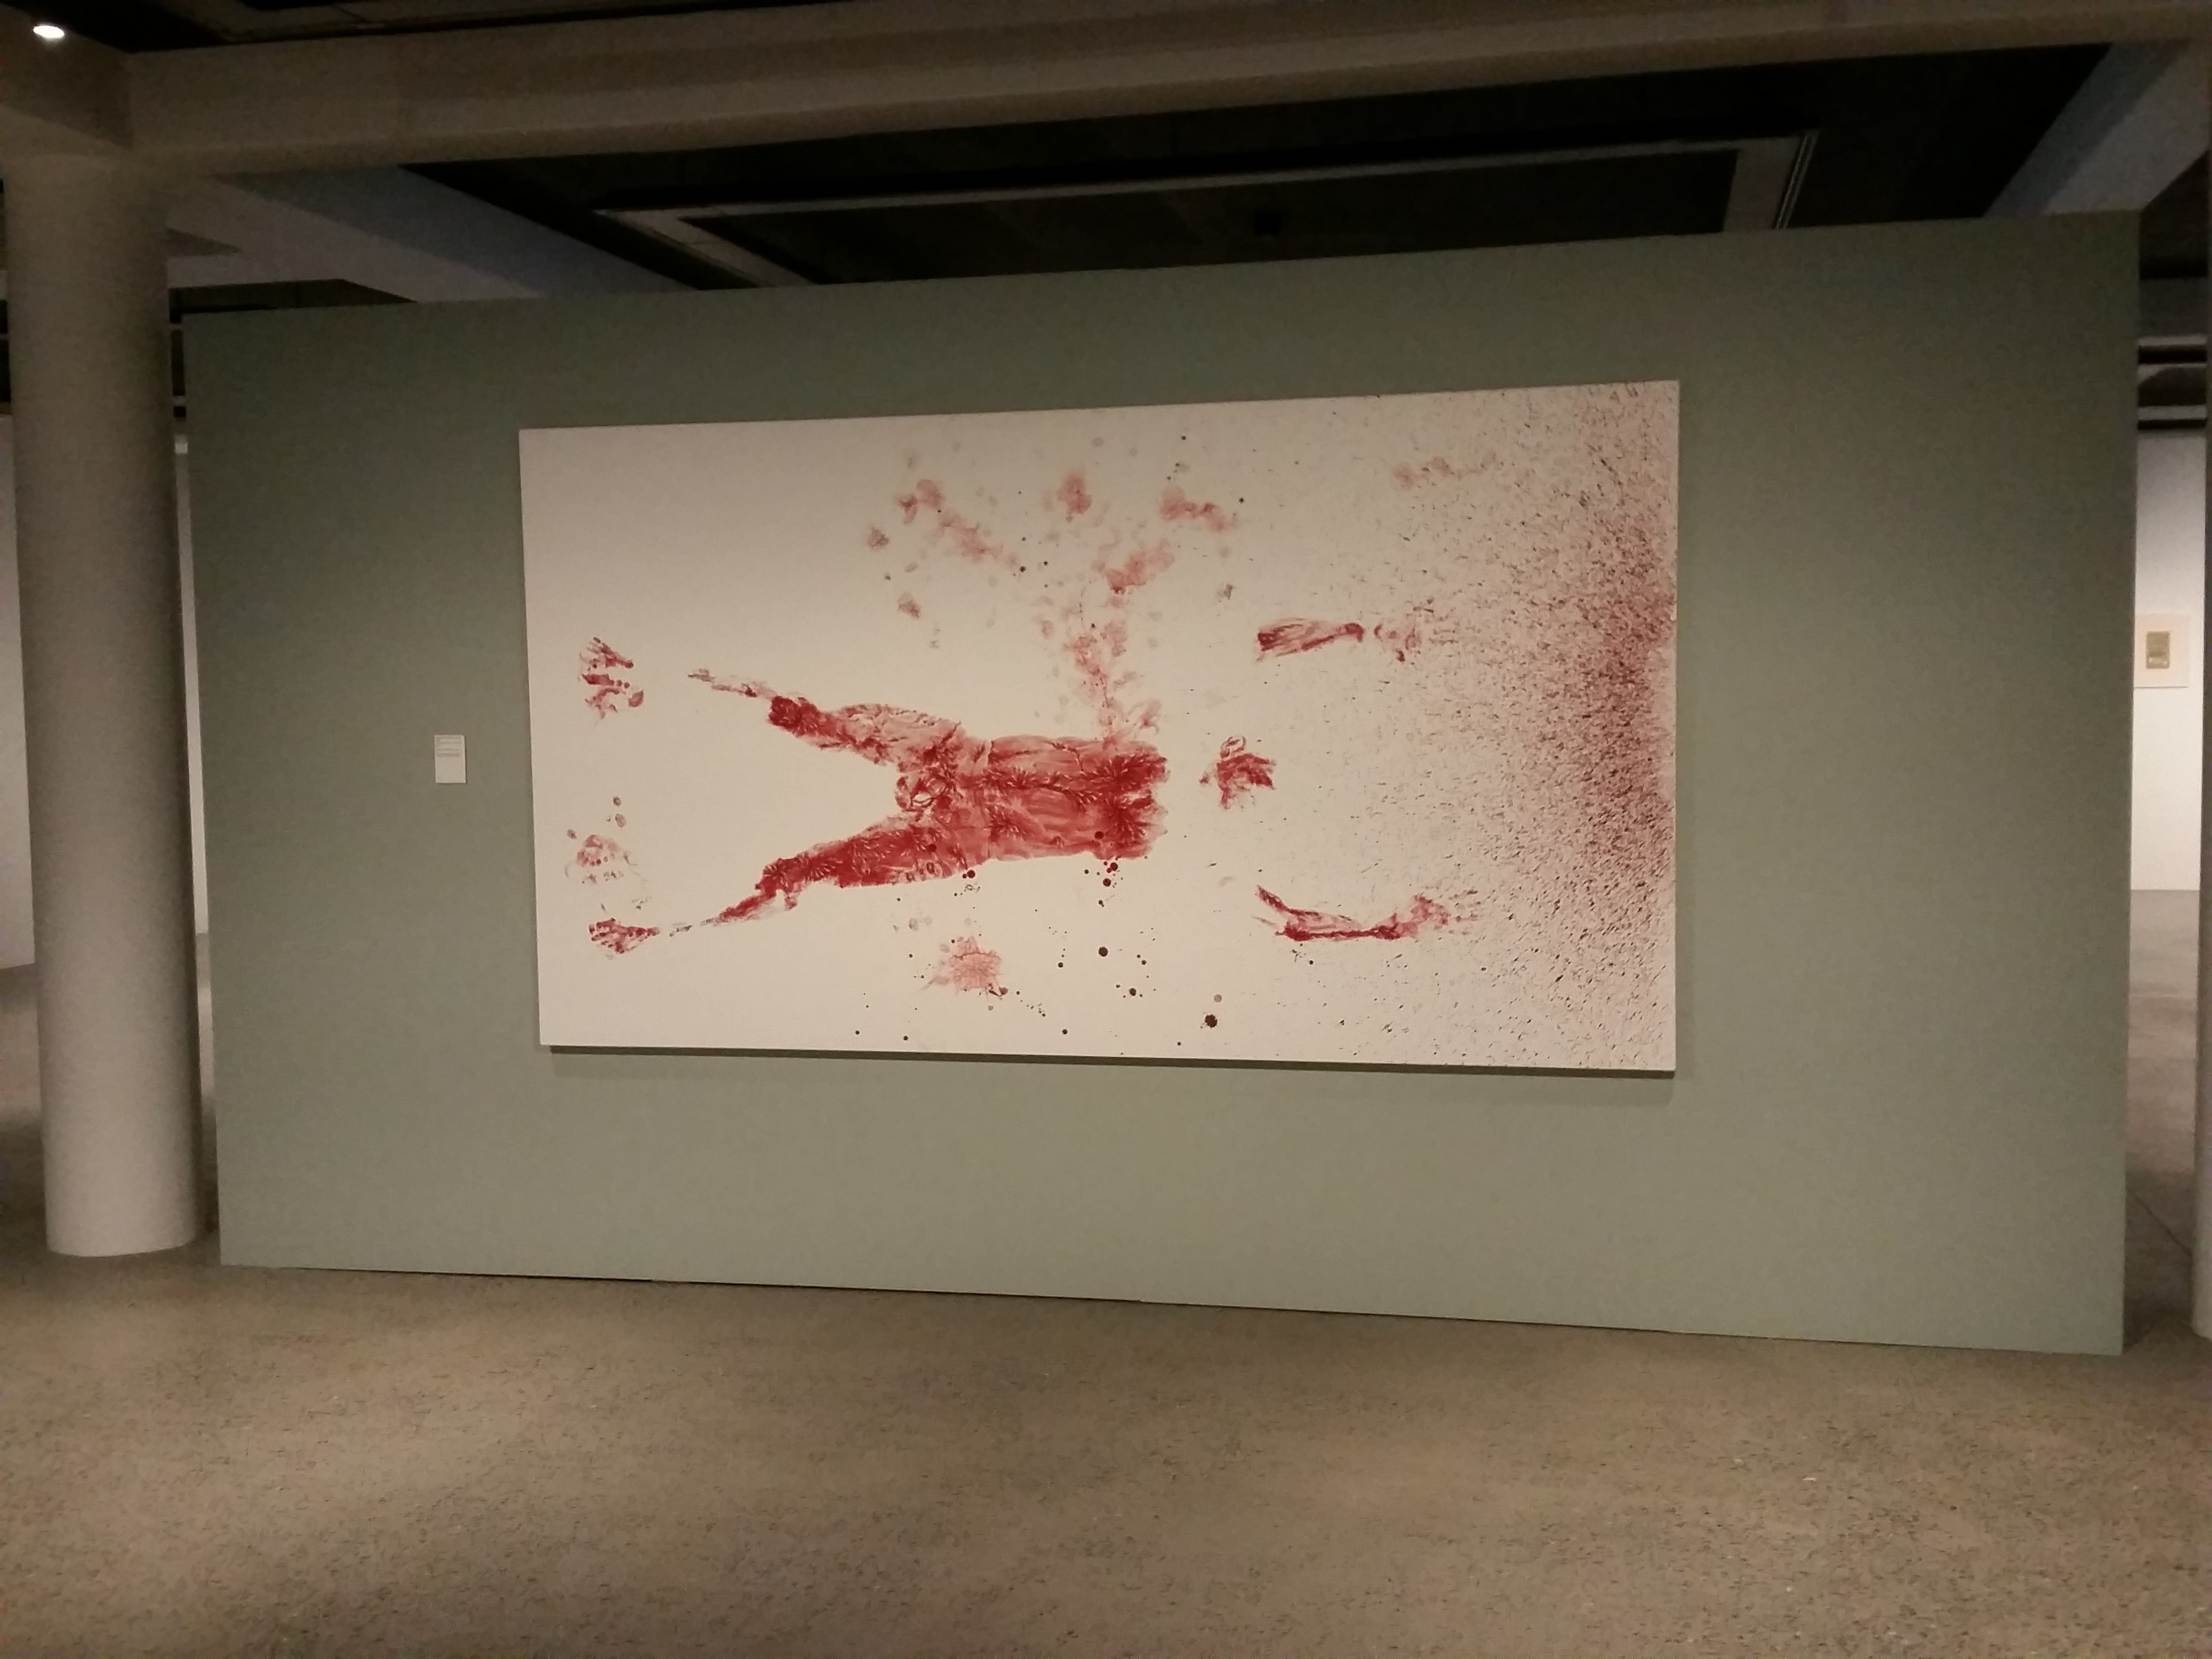
\includegraphics[width=1\textwidth]{aftryk}
\caption{\label{fig:aftryk} Picture taken from Kunsten.}
\end{figure}
The art piece has its own isolated wall with no sharing of space with other art pieces. Since the main project deals with audio, it was decided that it would be optimal for the product to be isolated from other art exhibitions to not disturb the visitors with loud noises.
 
 \begin{figure}[!h] 
\centering
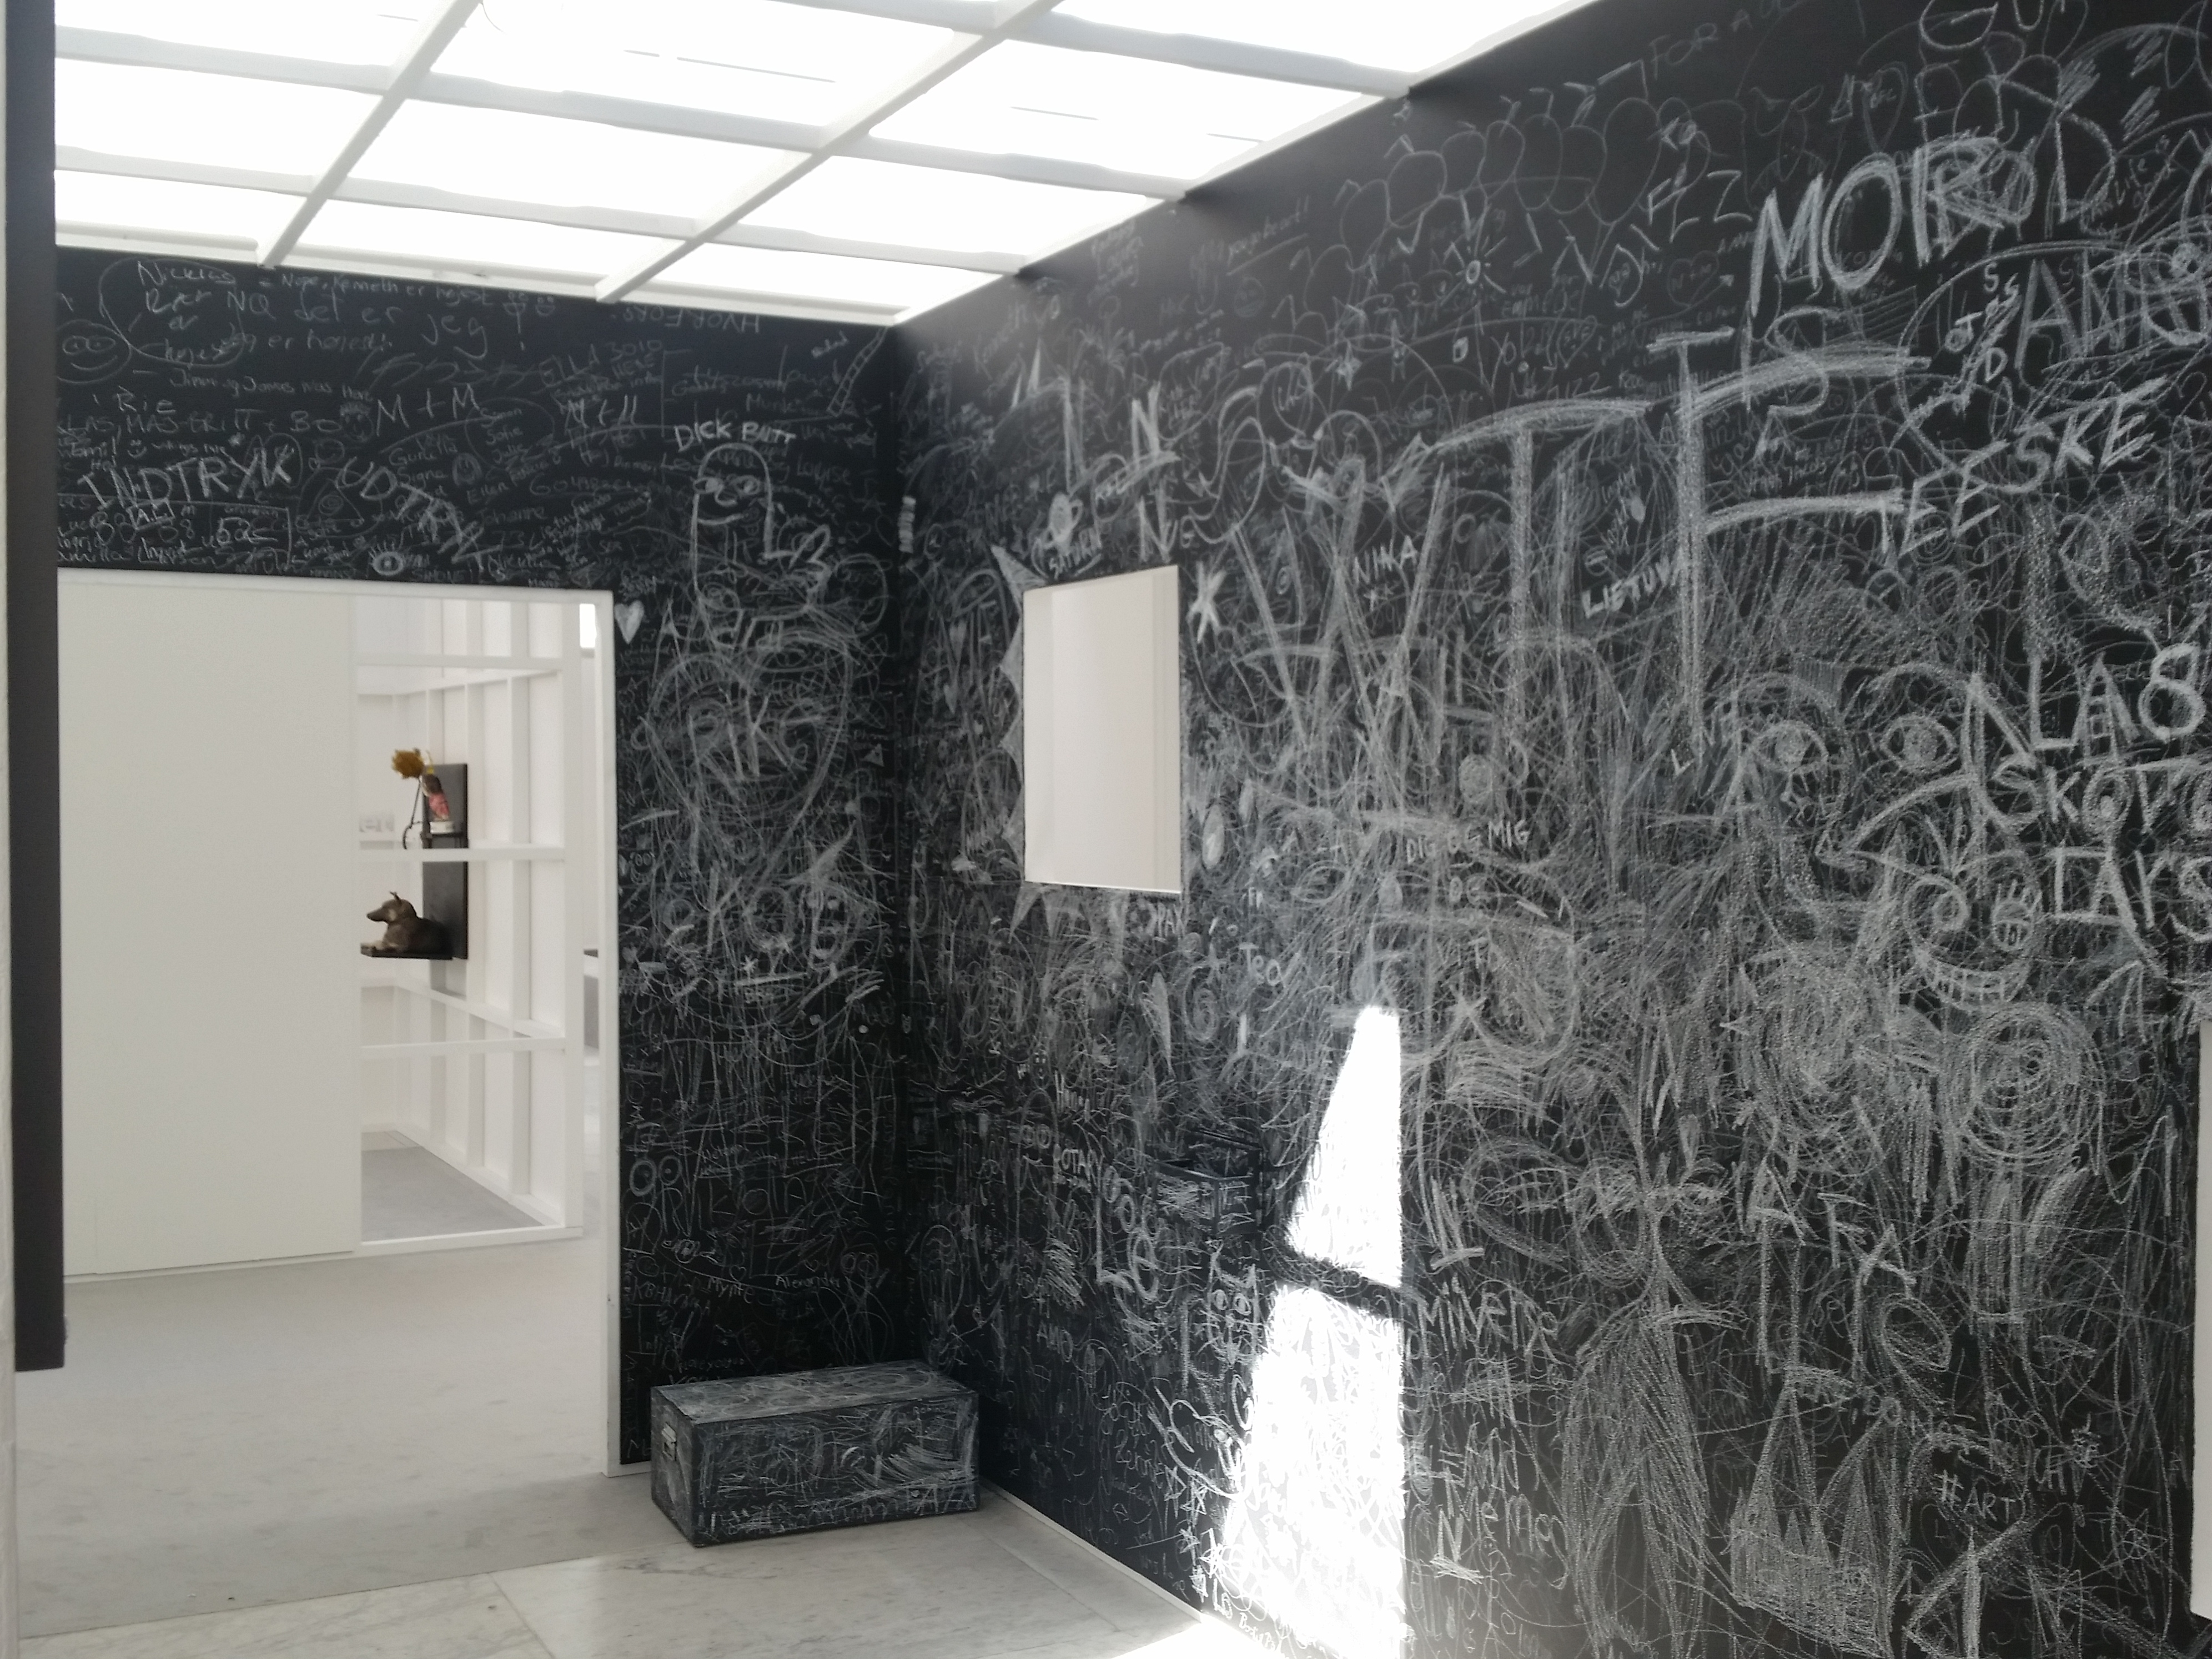
\includegraphics[width=1\textwidth]{chalk}
\caption{\label{fig:chalk} Picture taken from Kunsten.}
\end{figure}
This art piece has is own closed space and encourage the visitors to interact with it by drawing on the walls with white chalk. Since the main project is about making the people interact with our product \todo{help, don't know if this is correct enough} the project group took inspiration from this art piece. 

Results from the visit
The visit at Kunsten resulted in sketches of what the set up of the product could be like at an actual art museum  
 
 \begin{figure}[!h] 
\centering
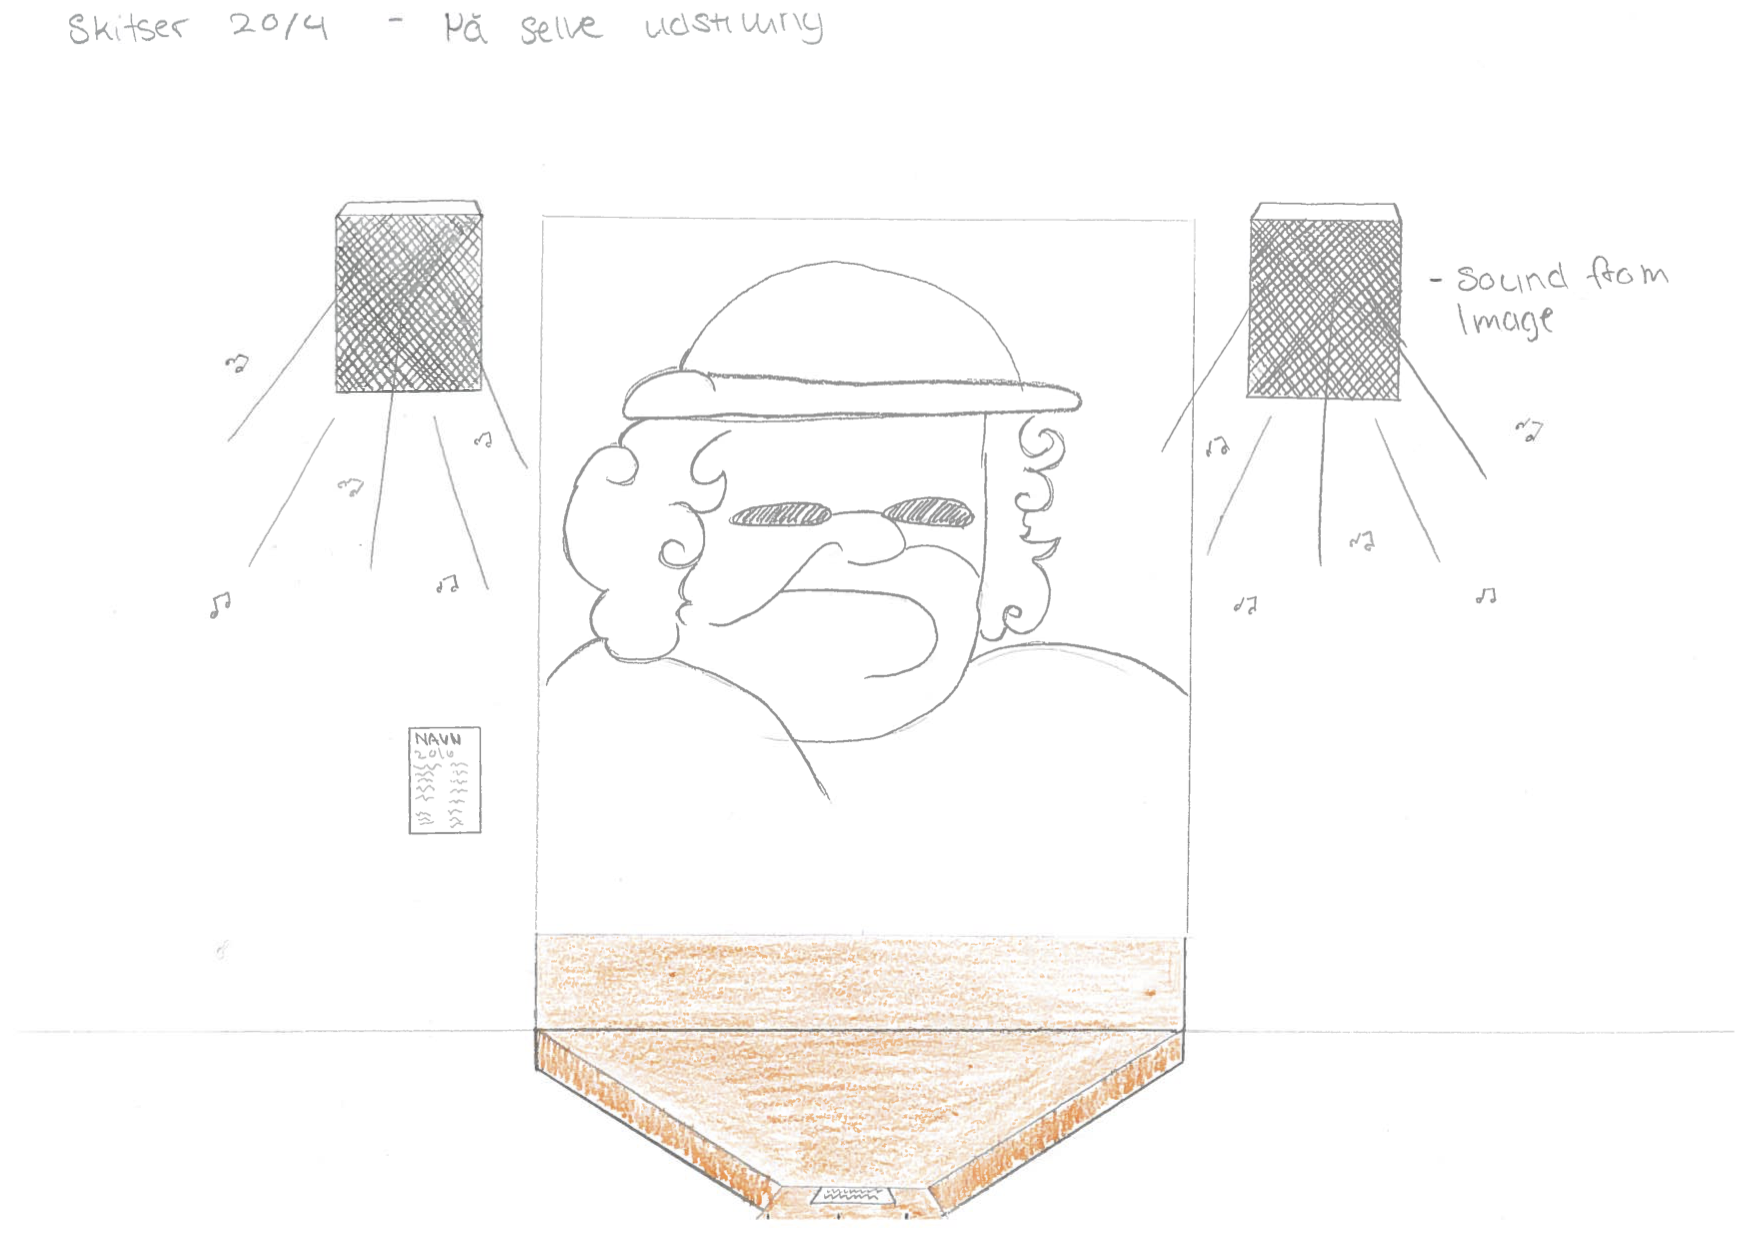
\includegraphics[width=1\textwidth]{productsetupsketch}
\caption{\label{fig:productsetupsketch} Sketch of an idea, on how to set up the product at an art museum.}
\end{figure}
 
 
\section{Wider context}
What can this be used for?

It would be possible to alter the function of the project, such that the user would have the possibility to decide where in the picture the program should be looking, as this would allow the user further freedom over the creation of sound, made by the product. But if it wasn't implemented correct, it would add to the confusion of the user, due to the amount of extra components on the interface. It could be done using an array of various components, such as a controller, slide potentiometers, or rotary encoders. 

Instead of choosing where in the picture to look, instead make it so that the user is able to create the picture being utilised by the software. This could allow the user to differentiate themselves from each other, and create unique and interesting sounds, increasing its potential as a creative tool for artists as well as non artists. This could also make it an entertaining product to have at things like festivals, events, or at a museum. 

An alternative version of the product, could be if instead of a picture, it worked with a video feed, allowing it to render and manipulate the information given in real-time. Allowing the user to translate his surrounding to sounds, giving a new perspective on the world, if this could be implemented onto a hand-held device, the user would be able to use things such as mobile phones or tablets. Which would allow the user to translate various areas without the need for a big machinery. 
The user could also have the possibility to upload their own pictures, videos, or even add their own sounds which are played when translating. 

portable version
During a discussion in the project group, it was suggested that the product could be used in other context like at a music or art festival. The idea was, that if the product should be should be presented at a festival, it had to have some changes to be suitable for the location. An idea was to make the product portable by putting it on wheels for easier transportation and elevate the electronic part of the product to prevent it from taking water and dirt in. In the figure \ref{fig:vidreudvikling} we see a sketch on how the portable version could look like. 

\begin{figure}[!h] 
\centering
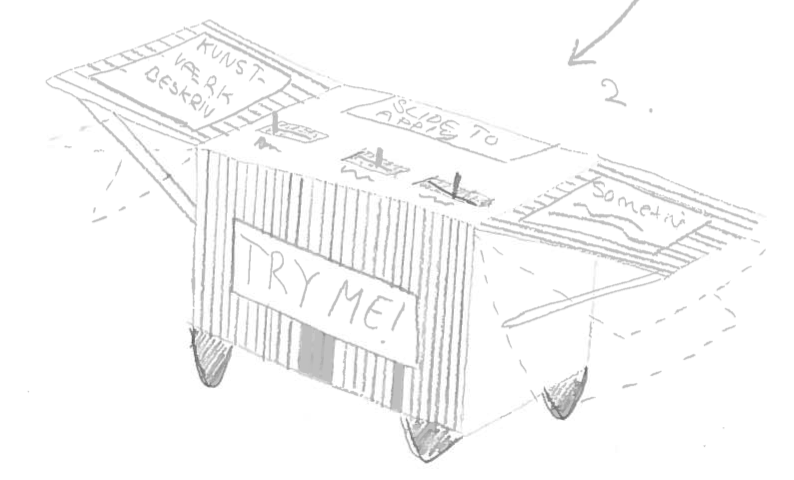
\includegraphics[width=0.5\textwidth]{vidreudvikling}
\caption{\label{fig:vidreudvikling} Sketch of how the portable version could look like.}
\end{figure}



\todo{additional functionality: draw on image to change the sound}

During the final test, one of the test participants was unsure of the connection between the artefact and the paintings shown during the test, he needed to be explained that the sound was made by the painting. Ideas were made to visualize the sound on the actual painting like shown in \ref{fig:Visualiseringaflyd} \todo{måske skald er tilføjes lidt mere, men ced ikke helt hvad}

\begin{figure}[!h] 
\centering
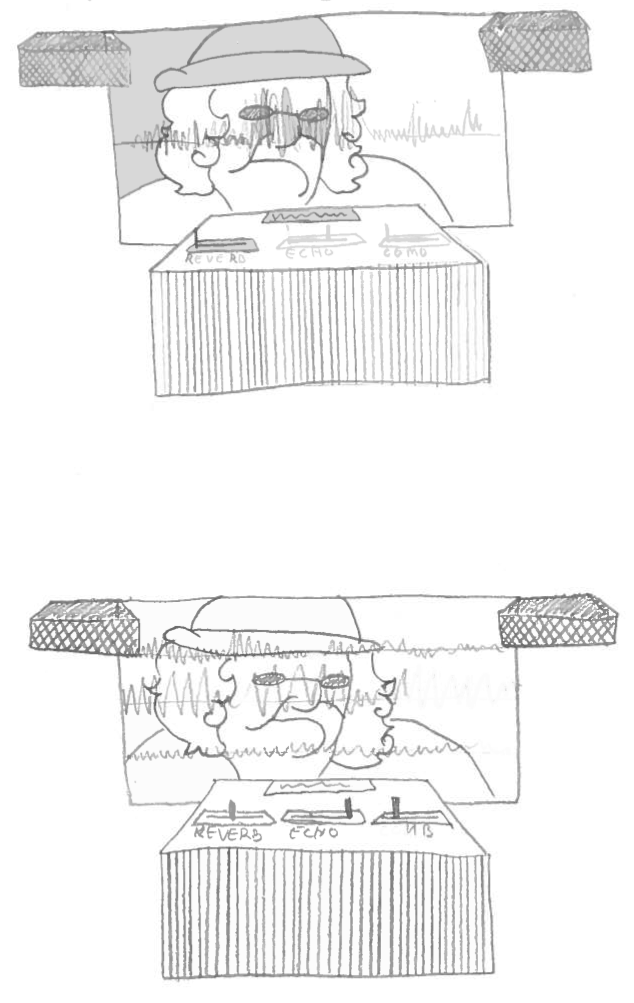
\includegraphics[width=0.5\textwidth]{Visualiseringaflyd}
\caption{\label{fig:Visualiseringaflyd} Sketch on how the sound could be visualized on the image.}
\end{figure}
 
 
